\documentclass[13pt]{beamer}
\usepackage{graphicx}
\usepackage[utf8]{inputenc}
 
% Formatting
\usetheme{Singapore}
\usecolortheme{whale}

% Title Page
\title{Geometric Manifolds and the Shape of Space}
\author{Devin Delfino}
\institute{MATH 331: Geometry}
\date{Fall 2014}

% Table of Contents
\setbeamertemplate{section in toc}[sections numbered]
\setbeamercolor{alerted text}{fg=blue}
\AtBeginSection[]
{
  \begin{frame}
    \frametitle{Outline}
    \tableofcontents[currentsection]
  \end{frame}
}
% \logo{\includegraphics[height=1.5cm]{lion-logo.png}}

\begin{document}
% TITLE ------------------------------------------------
\frame{\titlepage}

% Table of Contents ------------------------------------------------
\begin{frame}
\frametitle{Outline}
\tableofcontents
\end{frame}

\section{Geometric 2-Manifolds} % ==========================================================================
% TITLE ------------------------------------------------
\begin{frame}
\frametitle{Introduction}
	\begin{itemize}
		\item A \alert{Geometric 2-Manifold} is a connected surface that is locally isometric to either the Euclidean plane, hyperbolic plane, or sphere.
		\item Cones (excluding cone point), Cylinders, and Tori are examples of flat 2-manifolds
    \item The double torus is a 2-manifold that is locally isometric to the hyperbolic plane
	\end{itemize}
	\begin{columns}[r] % the "c" option specifies center vertical alignment
    \column{.3\textwidth} % column designated by a command
     \centering
     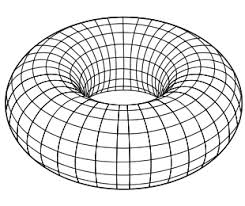
\includegraphics[height=2cm]{./img/torus}
    \column{.3\textwidth}
     \centering
     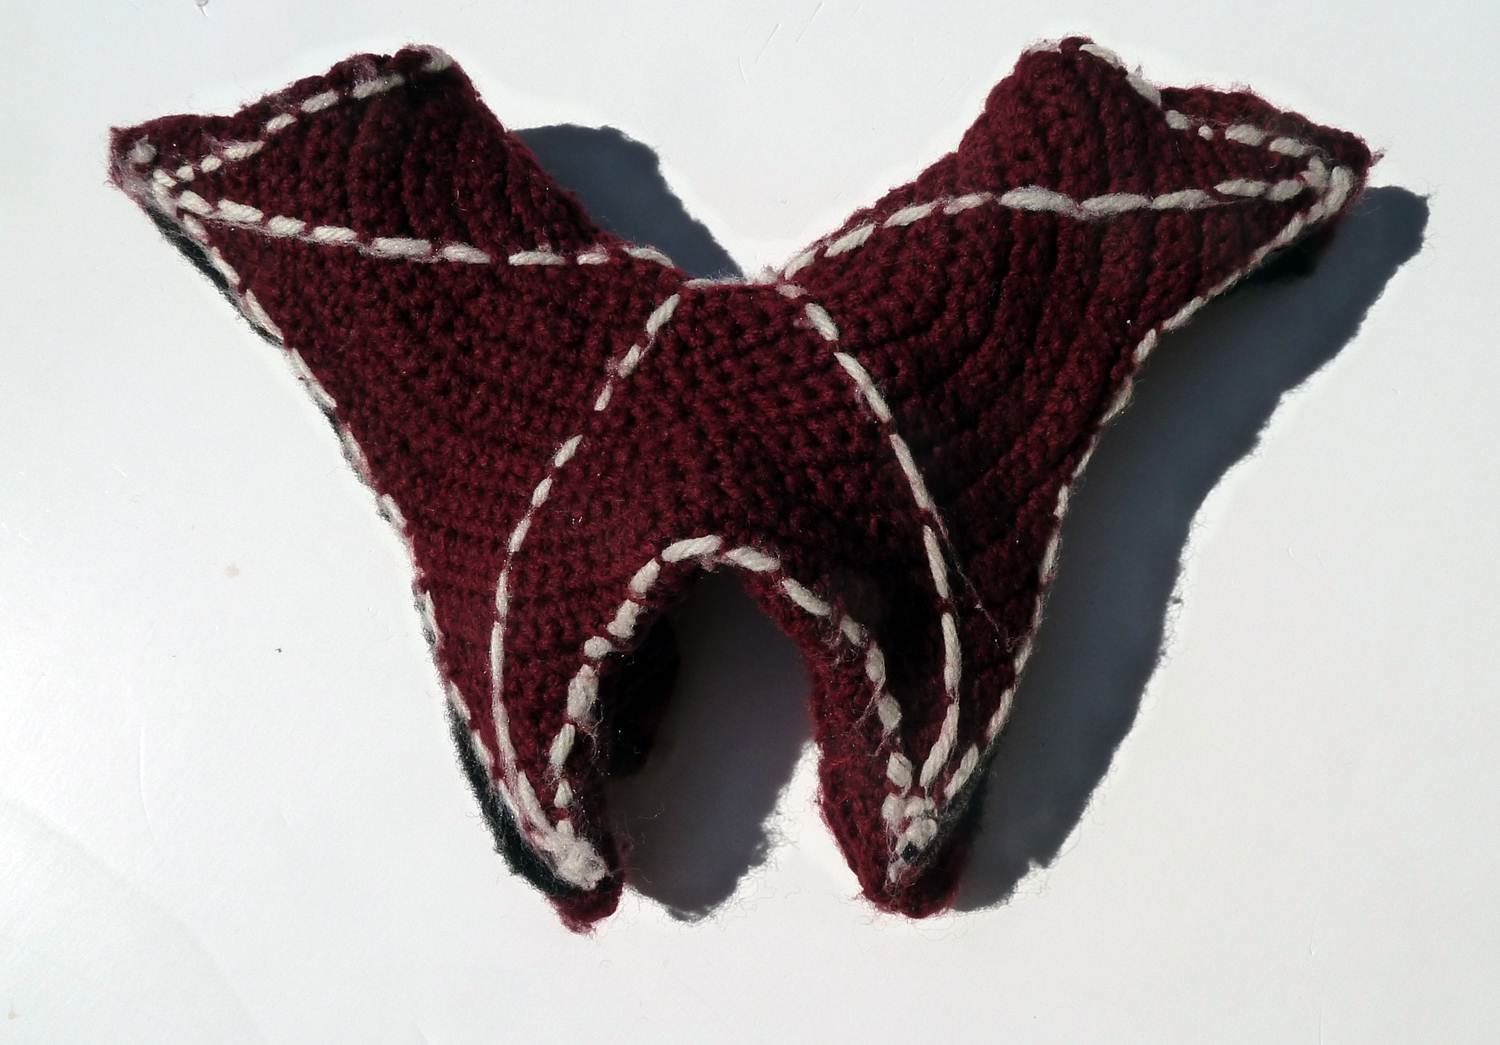
\includegraphics[height=2cm]{./img/hyperbolicpants}
    \column{.3\textwidth}
     \centering
     
\includegraphics[height=2cm]{./img/doubletorus}
  \end{columns}
	%torus, hyperbolic pants, double torus
\end{frame}

\begin{frame}
\frametitle{Gluings}
	\begin{itemize}
    \item \alert{Gluings} are when two edges or sides of a surface are ``connected'' and share the same set of points.
		\item The orientation of the gluings determine the structure of the manifold and whether it is flat, hyperbolic, or spherical.
	\end{itemize}

  \begin{columns}[r] % the "c" option specifies center vertical alignment
    \begin{column}{.5\textwidth} % column designated by a command
     \centering
     \begin{block}
      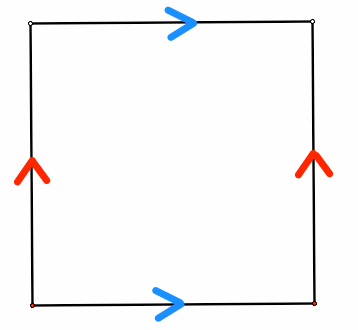
\includegraphics[height=2cm]{./img/torusgluing}
     \end{block}
    \end{column}
     % \begin{block}
     %  \includegraphics[height=2cm]{./img/coverings}
     % \end{block}
     % page 117 lower figure of shape of space
    \begin{column}{.5\textwidth}
     \centering
     \begin{block}
      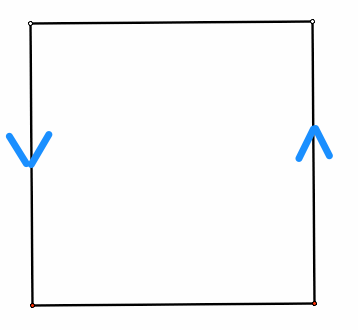
\includegraphics[height=2cm]{./img/mobiusgluing}
     \end{block}
     \begin{block}
      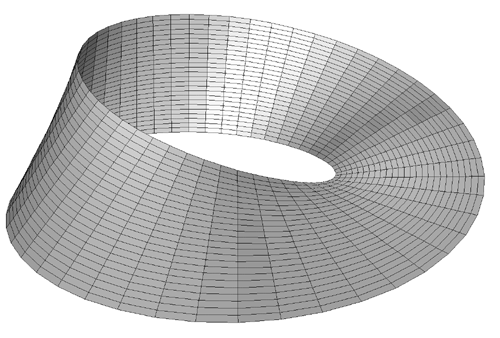
\includegraphics[height=2cm]{./img/mobius}
     \end{block}
     \end{column}
  \end{columns}
  % props- big torus, mobius strip
\end{frame}

\begin{frame}
\frametitle{Gluings}
	\begin{itemize}
		\item \alert{Gluings} are when two edges or sides of a surface are ``connected'' and share the same set of points.
		% gluings for torus, mobius strip
	\end{itemize}
\end{frame}

\section{Geometric 3-Manifolds} % ==========================================================================
% TITLE ------------------------------------------------
\begin{frame}
\frametitle{Geometric 3-Manifolds}
This is a text in first frame. This is a text in first frame. This is a text in first frame.
\end{frame}

\section{Cosmic Microwave Radiation} % ==========================================================================
% TITLE ------------------------------------------------
\begin{frame}
\frametitle{Cosmic Microwave Radiation}
This is a text in first frame. This is a text in first frame. This is a text in first frame.
\end{frame}

\section{The Shape of Space} % ==========================================================================
% TITLE ------------------------------------------------
\begin{frame}
\frametitle{The Shape of Space}
This is a text in first frame. This is a text in first frame. This is a text in first frame.
\end{frame}

% References ------------------------------------------------
 \begin{frame}[allowframebreaks]
  \frametitle{References}    
  \begin{thebibliography}{10}    
  \beamertemplatebookbibitems
  \bibitem{Autor1990}
    A.~Autor.
    \newblock {\em Introduction to Giving Presentations}.
    \newblock Klein-Verlag, 1990.
  \beamertemplatearticlebibitems
  \bibitem{Jemand2000}
    S.~Jemand.
    \newblock On this and that.
    \newblock {\em Journal of This and That}, 2(1):50--100, 2000.
  \end{thebibliography}
\end{frame}

\end{document}